%!TEX TS-program = xelatex
%!TEX encoding = UTF-8 Unicode
\documentclass{icisfinal}
\usepackage{graphicx}
\usepackage{subcaption}
\graphicspath{ {imagenes/} }
\title{Redes en el Cerebro}
\researchtype{Redes}
\shorttitle{Redes en el Cerebro}
\track{Redes en el Cerebro}

\usepackage[hidelinks]{hyperref}
\addbibresource{references.bib}

\usepackage{tabularx}  % To have the table fill out the page
\usepackage{multirow}
\usepackage{setspace} % To doublespacing
\usepackage{caption}
\usepackage{float}

\captionsetup{width=0.8\linewidth}

\begin{document}
\author{Daniel Caicedo, Ignacio Chiapella, Miguel Guerrero, Juan Knebel}
\maketitle

\begin{table}[h!]
  \centering
  \LARGE
  \begin{tabularx}{\textwidth}{@{}*2{>{\centering\arraybackslash}X}@{}}
    \textbf{Daniel Caicedo}        & \textbf{Ignacio Chiapella} \\
    UAH & FCEyN   \\
    djcc710@gmail.com & ignacio.chiapella@gmail.com \\
    \\
    \textbf{Miguel Guerrero}        & \textbf{Juan Knebel} \\
    CUFM & FCEyN   \\
    miguelgh72@gmail.com & juanknebel@gmail.com \\
    \\
  \end{tabularx}
\end{table}

\begin{abstract}
%  Escribir resumen del articulo

  \emph{\textbf{Keywords: Redes, Grafos, Pesos, Louvain, Densidad, Sueño, Cerebro} }
\end{abstract}

\section{Introducción}
%!TEX TS-program = xelatex
%!TEX encoding = UTF-8 Unicode

El cerebro es el órgano encargado de controlar y regular de forma centralizada las funciones del cuerpo. Éste consta de regiones diferenciadas asociadas a determinadas facultades específicas como las mentales, comportamientos u operaciones cognitivas, que trabajan de forma sincronizada e integrándose para controlar todo nuestro organismo. Por ello, se trata de un órgano de gran importancia y cuya relevancia ha dado lugar a numerosos estudios tanto anatómicos como fisiológicos, así como de neuroimagen, para entender su funcionamiento, tanto en condiciones normales como en condiciones patológicas, e incluso en diferentes estados de conciencia (dormidos o despiertos).\\
En la última década venimos asistiendo al fuerte auge de lo que se está dando en llamar la \textbf{Neurociencia de redes}, esto es, el estudio de la conectividad de redes cerebrales, mediante técnicas procedentes de la teoría de grafos.\\
La teoría de redes complejas es una herramienta muy potente que permite estudiar el cerebro desde el punto de vista de una red compleja, de forma que los nodos representan neuronas individuales o grupos neuronales y los enlaces entre éstos pueden representar tractos neuronales (conectividad estructural), relaciones de dependencia estadística (conectividad funcional) o efectos causales que una región ejerce sobre otra (conectividad efectiva).
Este trabajo tiene como antecedente el realizado por Tagliazucchi y colaboradores (2013), donde se busca relacionar cambios en la modularidad de las redes construidas a partir de la señal de resonancia magnética funcional con los distintos estadíos del sueño. \\
Nuestro objetivo es analizar y explorar los cambios en estas redes en función de la profundidad del sueño (N1, N2 y N3) y también establecer comparaciones contra la actividad cerebral cuando un individuo está despierto. Cabe destacar, que en el trabajo realizado por Tagliazucchi su estudio se basó en 63 sujetos y el presente trabajo será realizado analizando a 18 de estos, apoyándonos en la teoría de grafos, en técnicas de Clustering y métodos como el de Louvain. 

\newpage
\section{Tarea 1: Visualización}
%!TEX TS-program = xelatex
%!TEX encoding = UTF-8 Unicode

Antes de comenzar el análisis correspondiente a los distintos estadios de sueño, vamos mostrar una serie de gráficos y medidas de centralidad que obtuvimos como consecuencia de calcular los promedios de todas las matrices por cada fase N1, N2, N3 y W.

Lo primero que obtuvimos fue un grafo pesado completo para cada fase. En este caso las aristas dibujadas no está en proporción a su peso ya que no podría apreciarse en este tipo de gráfico.

\begin{figure}[H]
    \centering
    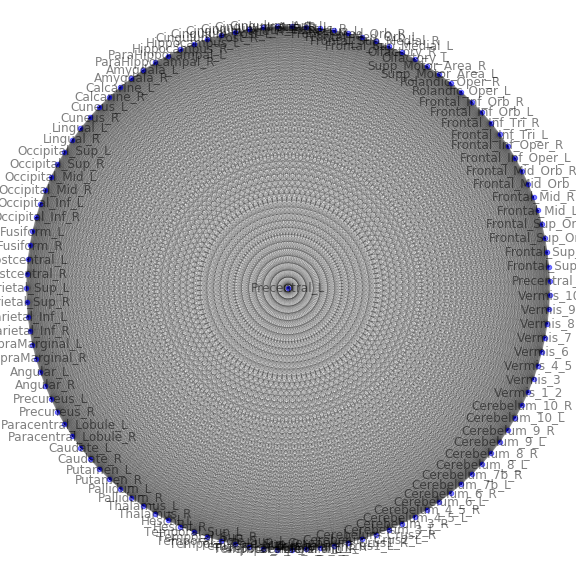
\includegraphics[width = 4in]{img/avg_w.png}
    \caption{Red del estadio W}
    \label{fig:avg-w}
\end{figure}

\begin{figure}[H]
    \centering
    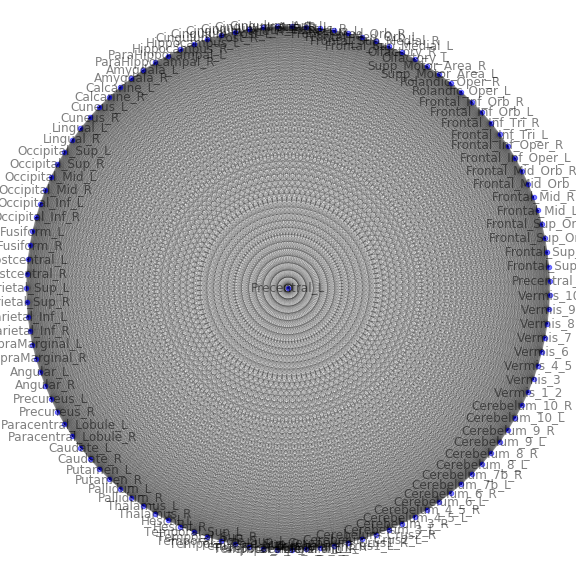
\includegraphics[width = 4in]{img/avg_n1.png}
    \caption{Red del estadio N1}
    \label{fig:avg-n1}
\end{figure}

\begin{figure}[H]
    \centering
    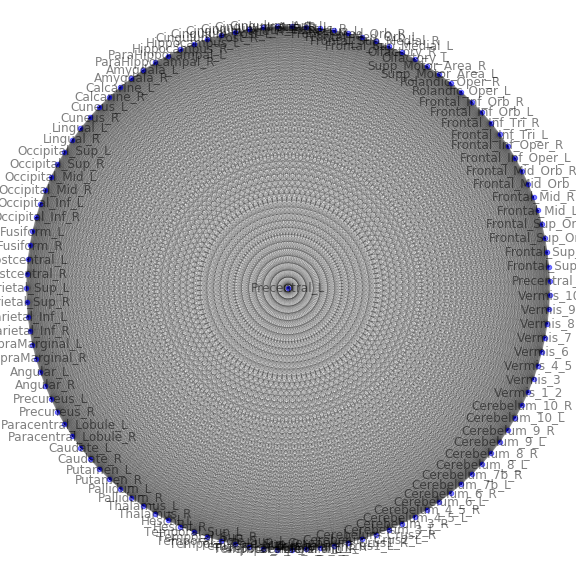
\includegraphics[width = 4in]{img/avg_n2.png}
    \caption{Red del estadio N2}
    \label{fig:avg-n2}
\end{figure}

\begin{figure}[H]
    \centering
    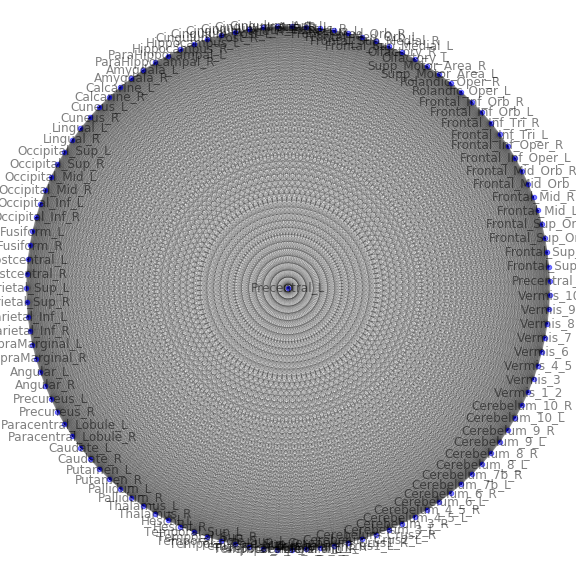
\includegraphics[width = 4in]{img/avg_n3.png}
    \caption{Red del estadio N3}
    \label{fig:avg-n3}
\end{figure}

Como mencionamos en el párrafo anterior, son grafos completos y en esta primera visualización no podemos extraer más información.

\subsection{Medidas de centralidad}
A continuación vamos a calcular algunas medidas de centralidad no para los grafos originales ya mencionados, sino sobre la transformación de los mismos a grafos no pesados y posteriormente tomando para de ellos subconjuntos de subgrafos en función de densidades previamente elegidas.

\begin{figure}[H]
    \centering
    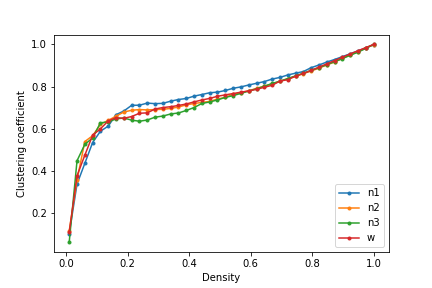
\includegraphics[width = 6in]{img/clust_coeff.png}
    \caption{Coeficiente de clustering}
    \label{fig:clust-coef}
\end{figure}

Se puede ver un crecimiento muy acelerado del coeficiente de clustering para los grafos de hasta una densidad de 0.2 del total de aristas, luego tal umbral el crecimiento se estanca y hasta disminuye para la fase \textbf{N3} pero la tendencia es en crecimiento pero con una pendiente muy pequeña.

\begin{figure}[H]
    \centering
    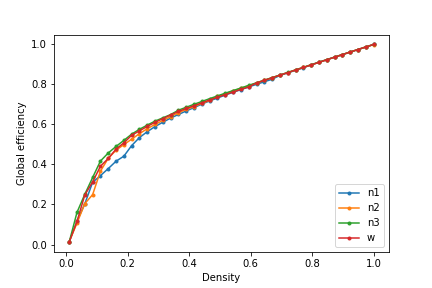
\includegraphics[width = 6in]{img/efficiency.png}
    \caption{Eficiencia}
    \label{fig:efficiency}
\end{figure}

Como para muchas de las densidades utilizadas se obtienen grafos que no son conexos, en lugar de usar el camino mínimo como medida de centralidad, utilizamos la medida de eficiencia global. La tendencia de las fases de sueño es creciente similar a una función logarítmica, salvo por \textbf{N1} que en todo momento se encuentra por debajo de las demás fases.

\begin{figure}[H]
    \centering
    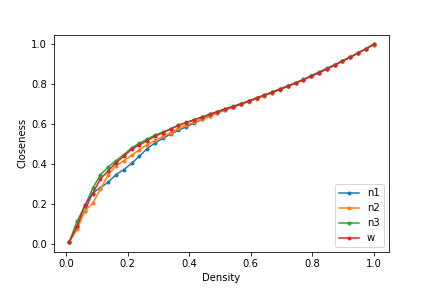
\includegraphics[width = 6in]{img/closeness.png}
    \caption{Cercanía}
    \label{fig:closeness}
\end{figure}

La medida de centralidad de cercanía también parece crecer muy rápidamente para las primeras densidades y luego el mismo crece casi linealmente.

\begin{figure}[H]
    \centering
    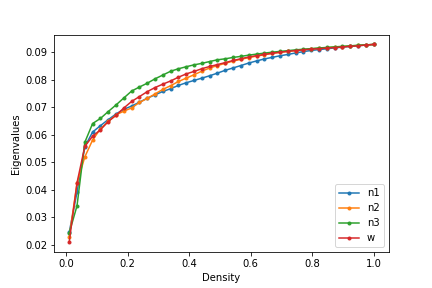
\includegraphics[width = 6in]{img/eigenvector.png}
    \caption{Autovalores}
    \label{fig:eigen}
\end{figure}

Para terminar observamos la medida de autovalores para las distintas densidades y se aprecia que también en las primeras densidades aumenta muy rápidamente y luego continúa el crecimiento pero con una acelaración mucho menor.

\begin{figure}[H]
    \centering
    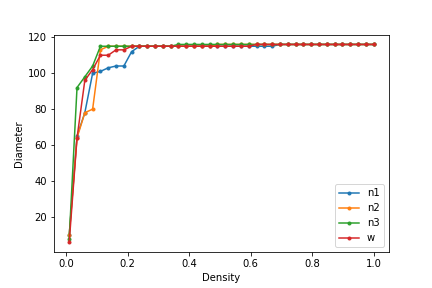
\includegraphics[width = 6in]{img/diameter.png}
    \caption{Diámetro}
    \label{fig:diameter}
\end{figure}

Para terminar calculamos el diámetro para las distintas densidades, como en algunos cortes se obtienen grafos no conexos, en esos casos decidimos graficar el máximo de los diámetros todas las componentes conexas de cada grafo. Aproximadamente se puede ver que ya para una densidad cercana al 0.3, se obtienen grafos fuertemente conectados \textbf{N2} y \textbf{N3} y para \textbf{N1} y \textbf{W} con menos de 3 componentes conexas. Como puede verse ya para la densidad de 0.7 todas las fases del sueño presentan un grafo fuertemente conexo.

\subsection{Visualización de comunidades}
Elegimos 4 densidades para visualizar como se agrupan los nodos de acuerdo a sus conexiones.

\begin{figure}[H]
    \centering
    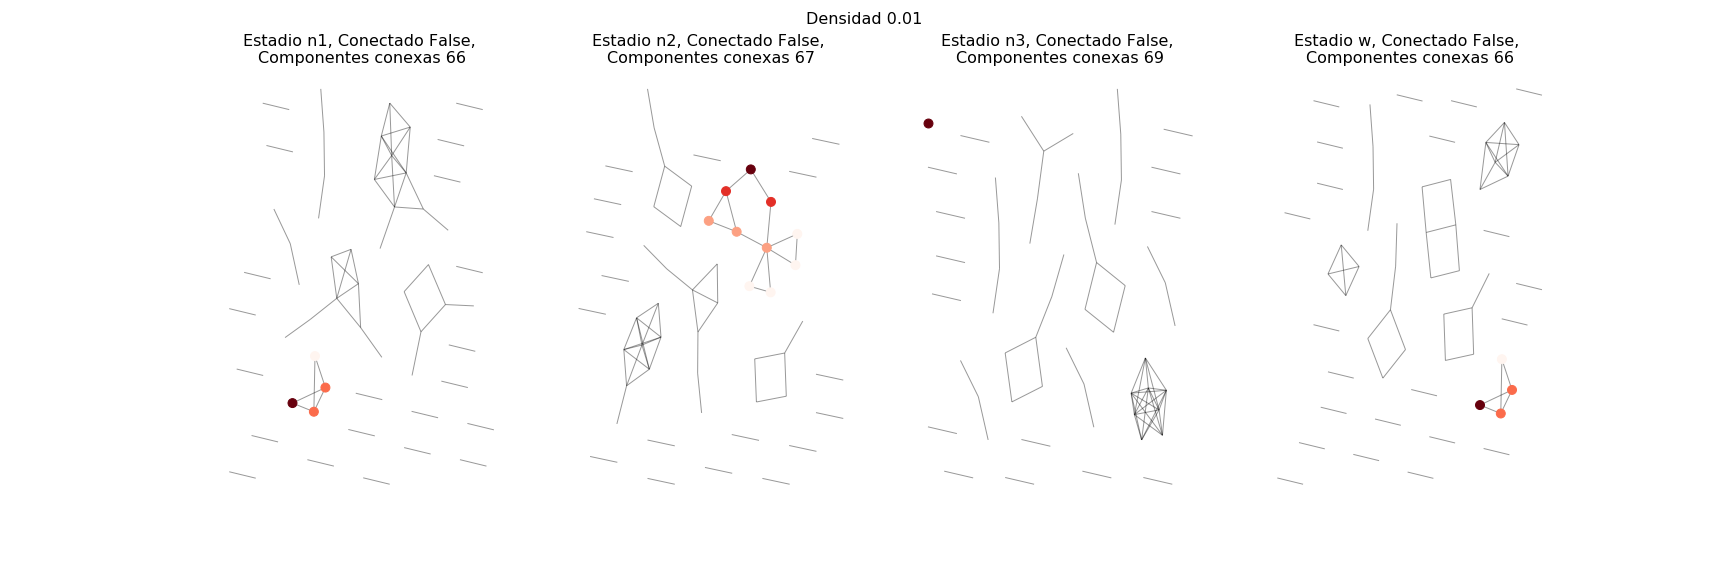
\includegraphics[width = \textwidth]{img/unweight_graphs_001.png}
    \caption{Estadios para densidad 0.01}
    \label{fig:unweight-001}
\end{figure}

En este caso se ve como todos los estadios tienen muchas componentes conexas y poca conexión entre ellas mismas.

\begin{figure}[H]
    \centering
    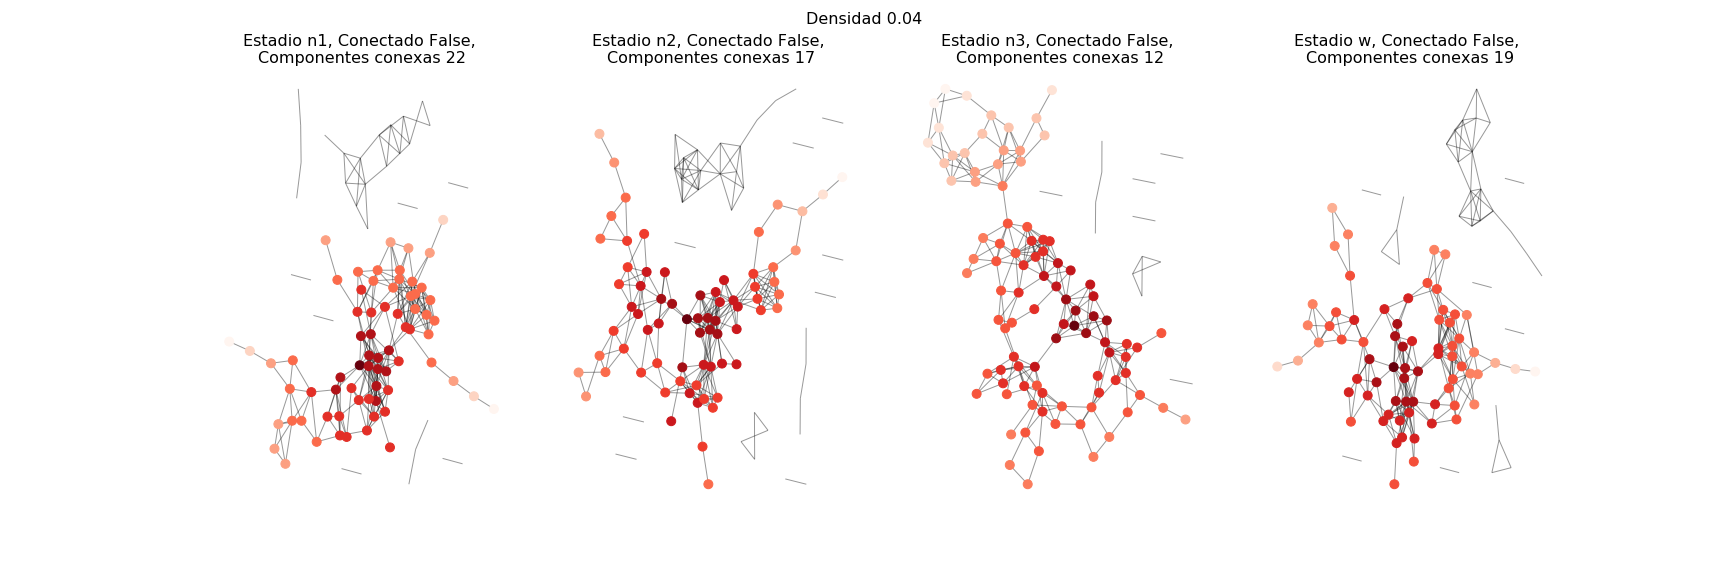
\includegraphics[width = \textwidth]{img/unweight_graphs_004.png}
    \caption{Estadios para densidad 0.04}
    \label{fig:unweight-004}
\end{figure}

Ya en esta etapa se ve que los nodos están mucho mas relacionados entre sí y la fase \textbf{N3} es la más conectada.
\begin{figure}[H]
    \centering
    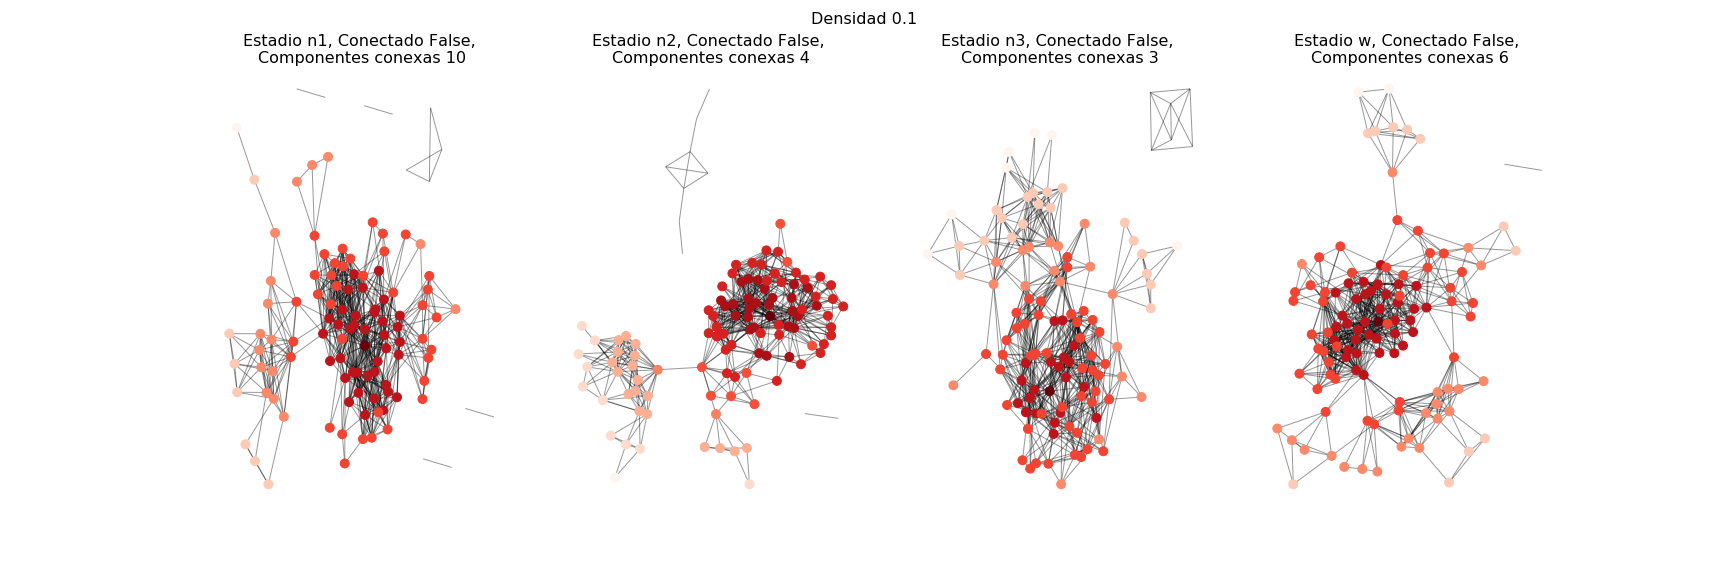
\includegraphics[width = \textwidth]{img/unweight_graphs_01.png}
    \caption{Estadios para densidad 0.1}
    \label{fig:unweight-01}
\end{figure}

En este corte solo el estadio \textbf{N1} tiene más de 10 componentes conexas, en cambio para \textbf{N2}, \textbf{N3} y \textbf{W} se observan grandes comunidades conectadas por algunas aristas entre ellas.

\begin{figure}[H]
    \centering
    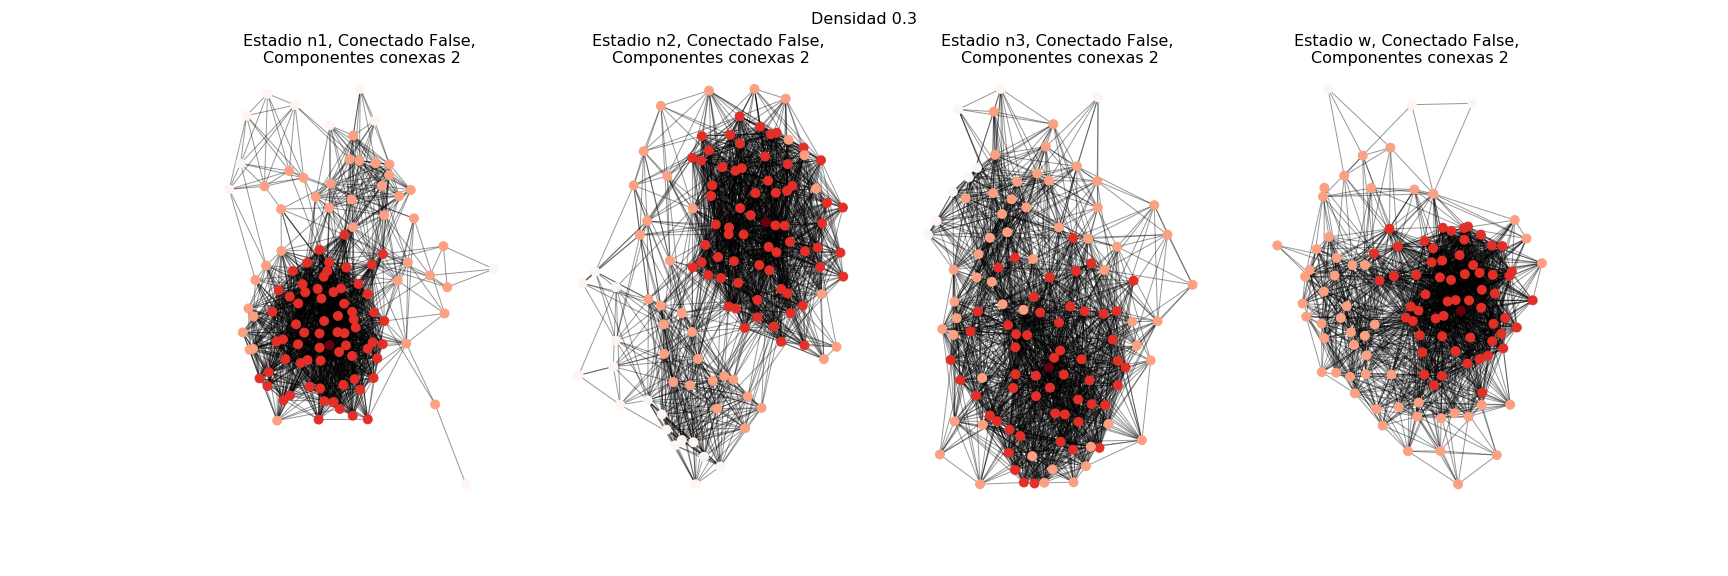
\includegraphics[width = \textwidth]{img/unweight_graphs_03.png}
    \caption{Estadios para densidad 0.3}
    \label{fig:unweight-03}
\end{figure}

Para finalizar en esta última densidad elegida, se puede observar que en todos los estadios el nodo asilado es el mismo el número 115, en \textbf{N3} se puede apreciar un único agrupamiento de nodos, en \textbf{N2} se ven dos grupos definidos y conectados entre ellos, mientras que en \textbf{N1} y \textbf{W} se observa un gran grupo conectado con otros más pequeños.

\newpage
\section{Tarea 2: Comunidades y coeficiente de modularidad}
%!TEX TS-program = xelatex
%!TEX encoding = UTF-8 Unicode



Basandonos en el algoritmo de Louvain para la conformacion de clusters es que comenzamos el analisis para cada estadio del sueño (W, N1, N2 y N3) y se calculó el promedio de las matrices de adyacencia de los 18 sujetos informados en el dataset.
Utilizando las distintas densidades de aristas fuimos creando grafos no pesados, para luego aplicar el algoritmo de clustering.

Para estudiar los resultados, se eligieron dos medidas de clustering \textbf{el coeficiente de modularidad y el número
de comunidades o módulos encontrados}


\begin{figure}[H]
    \centering
    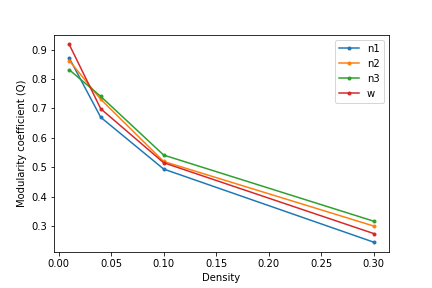
\includegraphics[width=\textwidth]{img/2_mod_coeff.png}
    \caption{Coeficiente de modularidad (Q) en función de las densidades}
    \label{fig:2_mod_coeff}
\end{figure}

Se observa que \textbf{Q} se decrementa en todos los casos a medida que la \textbf{densidad} aumenta. A partir de una \textbf{densidad = 0.15} la tendencia evidencia que los estadios se comportan asintoticamente y con una tendencia a la baja siendo \textbf{n3 > n2 > w > n1}.


\begin{figure}[H]
    \centering
    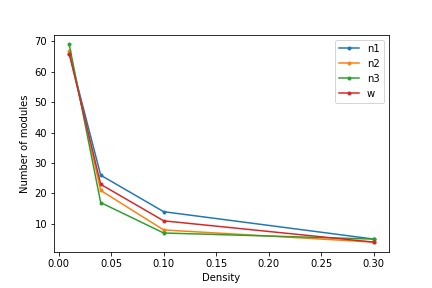
\includegraphics[width=\textwidth]{img/2_number_mod.png}
    \caption{Número de comunidades (Nc) en función de las densidades}
    \label{fig:2_number_mod}
\end{figure}

El numero de \textbf{comunidades} se decrementa fuertemente en el intervalo que va de 0 a 0.10 de la densidad. Luego siguen disminuyendo pero a una velocidad menor pero con una tendencia sostenida que permite afirmar que al igual que con el \textbf{Q}, a mayor \textbf{densidad} menor numero de \textbf{comunidades}.




\subsection{Redes Random}

Se vuelven a hacer los estudios anteriores pero esta vez comparando las distintas medidas de clustering contra una red random que preserva la distribución de grados de los nodos.


\begin{figure}[H]
    \centering
    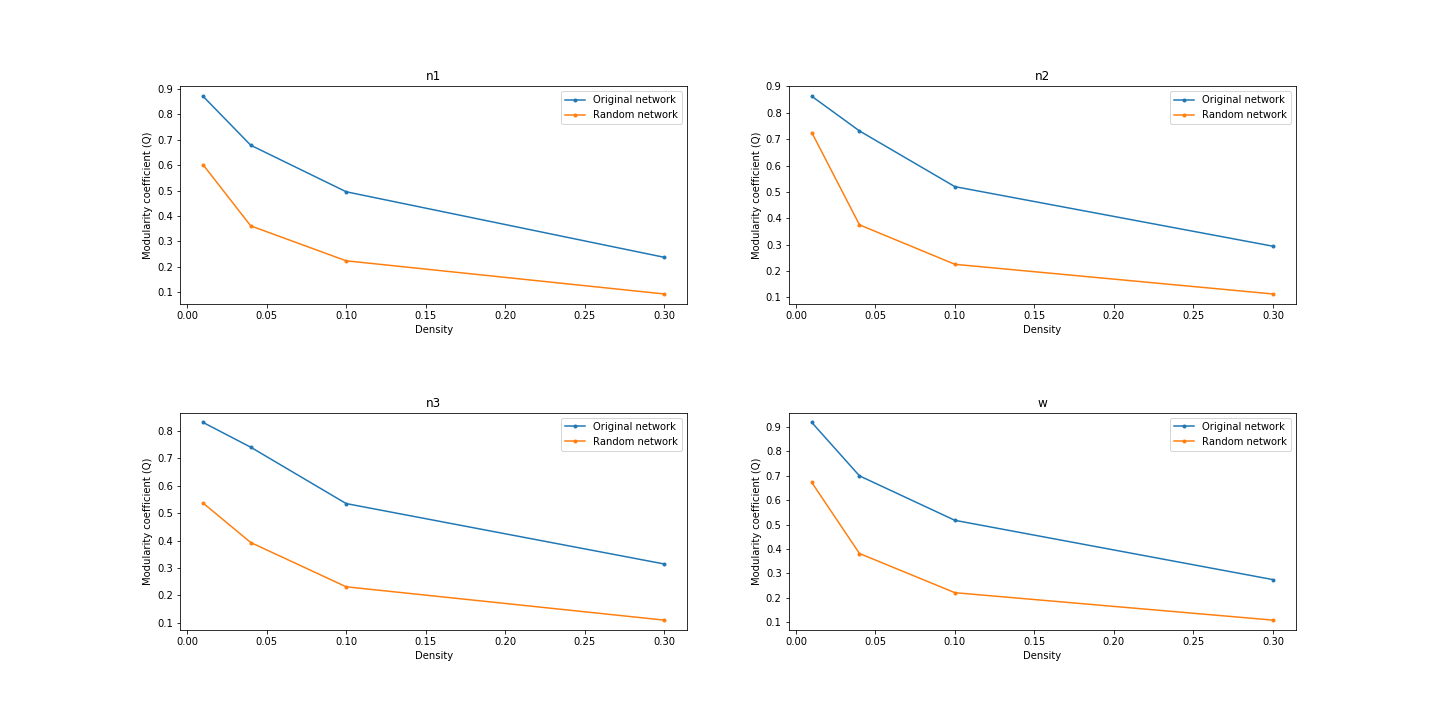
\includegraphics[width=\textwidth]{img/2_mod_coeff_vs_random.png}
    \caption{Red original vs Random - coeficiente de modularidad (Q) en función de las densidades}
    \label{fig:2_mod_coeff_vs_random}
\end{figure}

Al estudiar por separado los cuatro estadios del sueño y compara el \textbf{Q} tanto para la red original vs una red random, podemos observar que la red random muentra en todos los casos valores menores de \textbf{Q} para una densidad dada, pero conserva la misma tendencia de la red original de decrecer el \textbf{Q} a medida que aumenta la \textbf{densidad}




\begin{figure}[H]
    \centering
    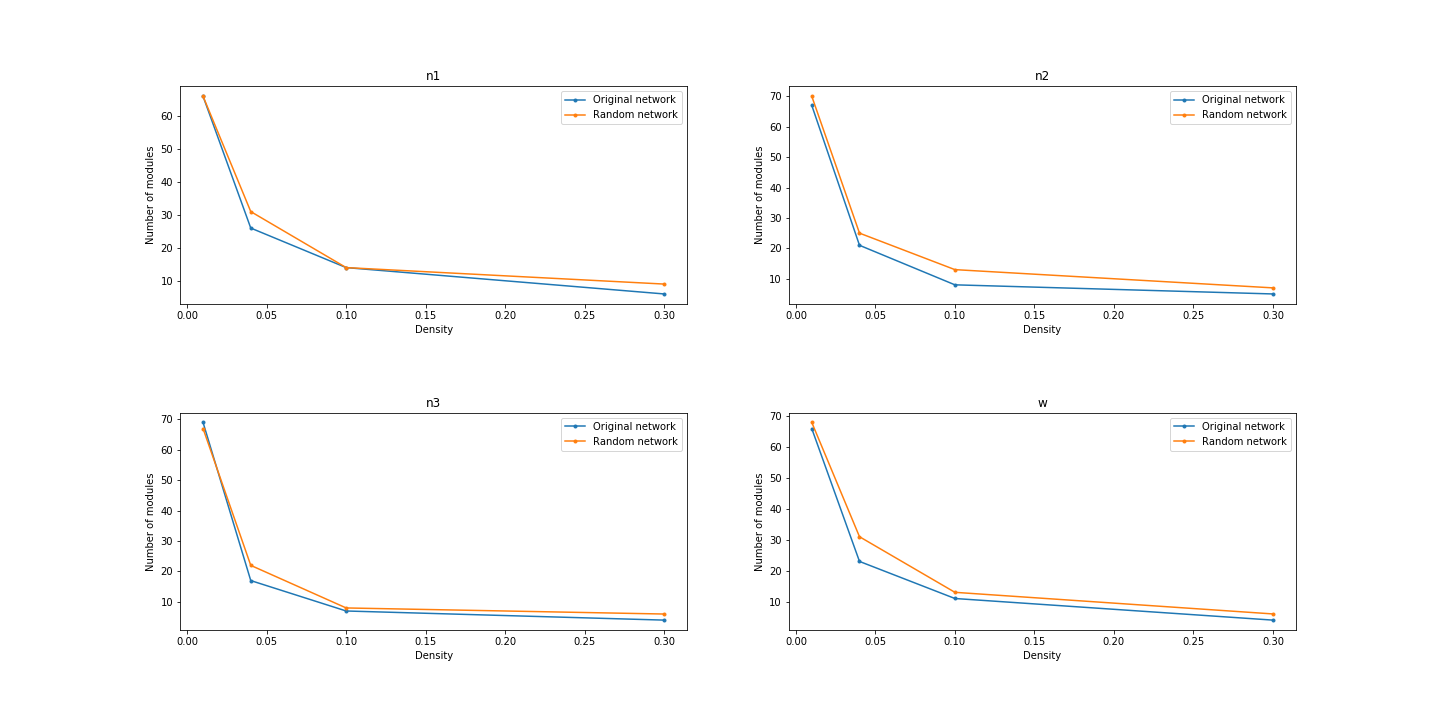
\includegraphics[width=\textwidth]{img/2_number_modules_vs_random.png}
    \caption{Red original vs Random - Número de comunidades (Nc) en función de las densidades}
    \label{fig:2_number_modules_vs_random}
\end{figure}


Para el caso de las \textbf{comunidades}, si bien la tendencia es la misma que la enunciada con anterioridad, en este caso la red random muesta valores de comunidades ligeramente mayores o iguales que la red original. Para el caso del estadio $n3$ y en especial el $n1$ las curvas se igualan en algunos puntos.

\newpage
\section{Tarea 3: Estadística + Opcional 2 (Tarea 3)}
%!TEX TS-program = xelatex
%!TEX encoding = UTF-8 Unicode


En el siguiente punto se pueden observar las curvas de modularidad \textbf{(Q)} y número de comunidades \textbf{(NC)} por cada sujeto y para cada estadio del sueño, en lugar de utilizar las matrices promedio como en el punto anterior.

En primer lugar, se aplicó el metodo de Louvain y se obtuvieron los coeficientes de modularidad y el número de comunidades, posteriormente se realizan las comparaciones del estado W contra los estados del sueño N1, N2 y N3 con un t-test, donde analizando los resultados se observó la necesidad de realizar corrección por comparaciones multiples debido a la alta probabilidad de ocurrencia de falsos positivos.

Posteriormente, para realizar la corrección por comparaciones multiples, se realizó un test de ANOVA mixto para los individuos y cada etapa del sueño. Los p valores de las densidades se calcularon con un test de Tukey para controlar la comparación de todos los grupos y se ajustaron siguiendo el método Benjamini-Hochberg.

\begin{figure}[H]
    \centering
    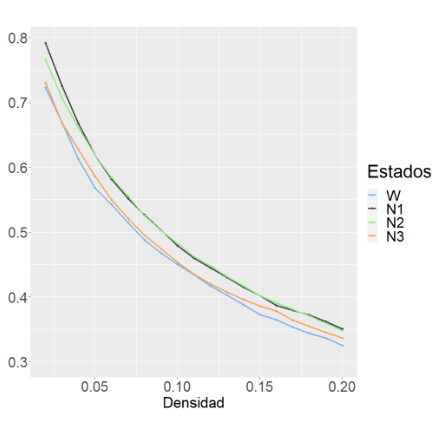
\includegraphics[width = 5in]{img/3_1_Modularidad.jpg}
    \caption{Modularidad}
    \label{fig:3_1_Modularidad}
\end{figure}

En el gráfico de modularidad, donde se comparan los estadíos N1, N2 y N3 contra el estadío W, se puede observar que W y N3 presentan una modularidad similar, sin embargo, los estadíos N1 y N2 presentan valores similares entre sí y una modularidad claramente mayor a W.

\begin{figure}[H]
    \centering
    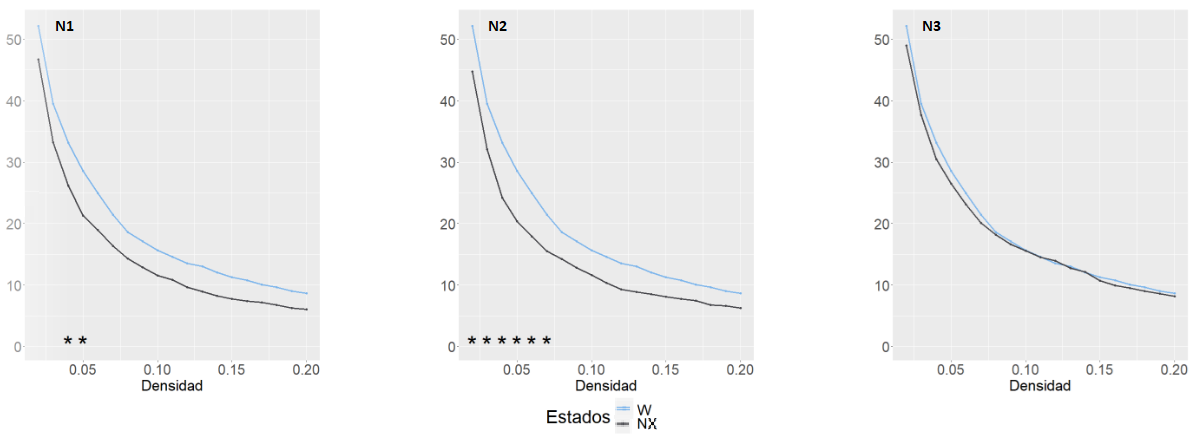
\includegraphics[width=\textwidth]{img/3_2_N_comunidades.jpg}
    \caption{Número de Comunidades}
    \label{fig:3_2_N_comunidades}
\end{figure}


En cuanto al número de comunidades, se repite un análisis similar al anterior, pero se grafica la comparación de cada estadío N1, N2 y N3 con W en gráficos distintos para observar los valores de densidad donde hay resultados significativos (identificados con asteriscos en la parte inferior del gráfico). Para cada estadío, se observa un comportamiento similar al visto en la modularidad, ya que N1 y N2 también presentan un número de comunidades superior a W y con respecto al estadío N3 este presenta valores muy similares a W.


\section{Tarea 4: Diferencias en la membresía para los diferentes estadíos}
%!TEX TS-program = xelatex
%!TEX encoding = UTF-8 Unicode

De acuerdo a lo especificado en la consigna, para cada valor de densidad, siguiendo  el procedimiento propuesto por Alexander-Bloch y colaboradores (Alexander-Bloch et al., 2012). Para cada par NX y W se calcula la similaridad entre grupos a partir de Índice de Rand Ajustado (adjusted-for-chance Rand index, ARI), y el valor promedio se compara con Np permutaciones de las etiquetas de comunidades para cada estadío. El p-valor se obtiene dividiendo el número de veces en que una permutación supera el valor promedio para los datos no permutados por el número total de permutaciones (Np).

El valor obtenido para cada densidad se compara con los que se obtienen de realizar 300 permutaciones de las membresías de uno de los estadíos. 

Se observan los resultados del p-valor con un $+$ en cada una de las figuras.


\begin{figure}[H]
    \centering
    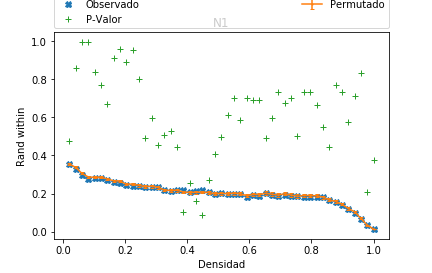
\includegraphics[width = 5in]{img/4_N1.png}
    \caption{N1}
    \label{fig:4_N1.png}
\end{figure}

\begin{figure}[H]
    \centering
    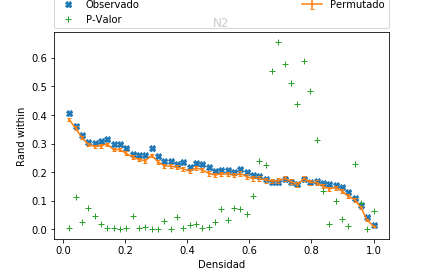
\includegraphics[width = 5in]{img/4_N2.png}
    \caption{N2}
    \label{fig:4_N2.png}
\end{figure}

\begin{figure}[H]
    \centering
    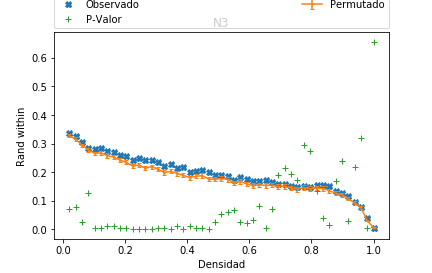
\includegraphics[width = 5in]{img/4_N3.png}
    \caption{N3}
    \label{fig:4_N3.png}
\end{figure}


Como conclusion de estos analisis podemos enunciar que las mayores diferencias en las membresías con respecto al estado \textbf{despierto} se registran en 
El estadío \textbf{N2} donde el índice de Rand inicia cerca del 0.4 y culmina muy cercano a 0 a medida que aumenta la densidad.

Destacamos que tanto en el estadío \textbf{N2} como el \textbf{N3}  se obtienen p-valores  significativos (0.05) lo cual no ocurre para el estadio \textbf{N1}.
No se observa una diferencia significativa entre los índices de Rand efectivos y los resultantes de las permutaciones.


\section{Opcional 5: Rol de nodos, y cambios en el rol de los nodos}
%!TEX TS-program = xelatex
%!TEX encoding = UTF-8 Unicode

En este ejercicio buscaremos una definición de roles de nodes dentro de las comunicades para así conocer aquellos que cambian de una comunidad a otra, cambian de rol dentro de la misma comunidad e incluso ubicar aquellos que contribuyen de manera positiva a mantener una buena comunicación entre distintas comunidades.
A cada nodo podemos asignarle un rol dentro de la red dependiendo de su conectividad dentro del módulo al que pertenece y su conectividad con el resto de las comunidades, luego de definir la estructura modular de la red (realizado mediante el algoritmo de Louvain). 
Comparamos la media de cantidad de nodos de cada rol en cada estadío del sueño contra el estadío ‘despierto’, para cada valor de densidad. Se hace una comparación estadística en la cual se observan muy pocas diferencias significativas.


\subsubsection{Connector Nodes}
La cantidad de Connector Nodes crece con el incremento de la densidad para todos los estadíos del sueño y para el estado despierto. No se hallaron diferencias significativas aunque para todos los casos los estadíos de sueño se observaron valores ligeramente más elevados que el estado despierto.


\begin{figure}[H]
    \centering
    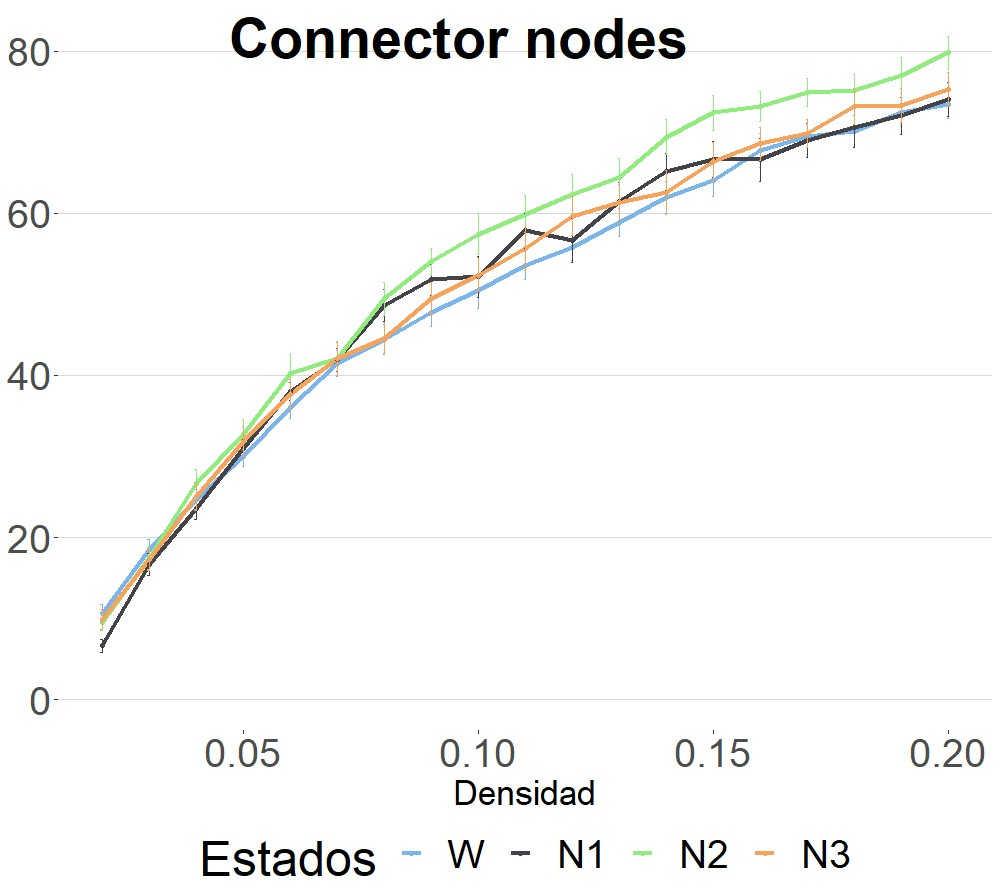
\includegraphics[width = 5in]{img/5_connectornodes.jpg}
    \caption{Connector Nodes}
    \label{fig:5_connectornodes}
\end{figure}

\subsubsection{Hubs}
La diferencia entre el estado despierto y las distintas etapas del sueño no resulta significativa en ningún caso. Puede observarse como la cantidad de hubs se incrementa a medida que se incrementa la densidad. El comportamiento resulta más similar entre W y N1 y N2 ya que muchas veces se cruzan sus trazas. El gráfico de W versus N3 presenta la mayor diferencia ya que la traza de N3 se encuentra siempre por encima de la de W.

\begin{figure}[H]
    \centering
    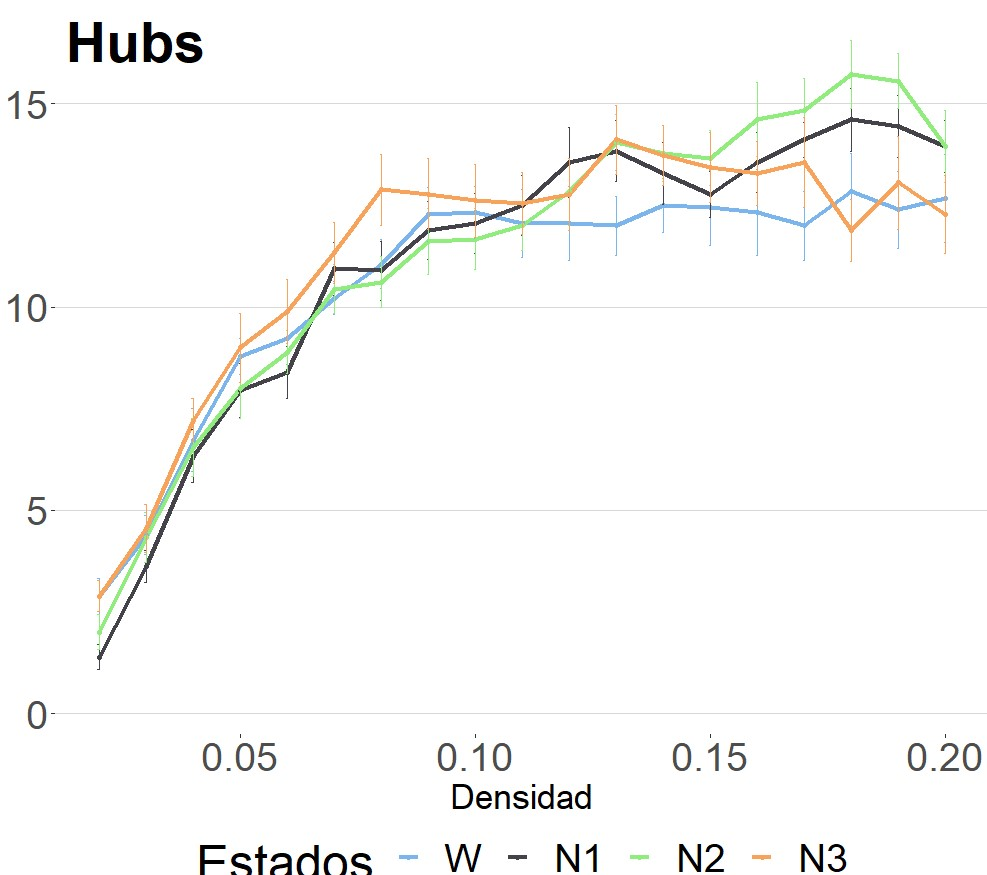
\includegraphics[width = 5in]{img/5_hubs.jpg}
    \caption{Hubs}
    \label{fig:5_hubs}
\end{figure}

\subsubsection{Provincial Hubs}
La cantidad de Provincial Hubs decrece con el incremento de la densidad para todos los estadíos del sueño y
para el estado despierto. Vemos que N1 se mantiene por encima de W en la mayoría de los puntos y N3 por debajo.

\begin{figure}[H]
    \centering
    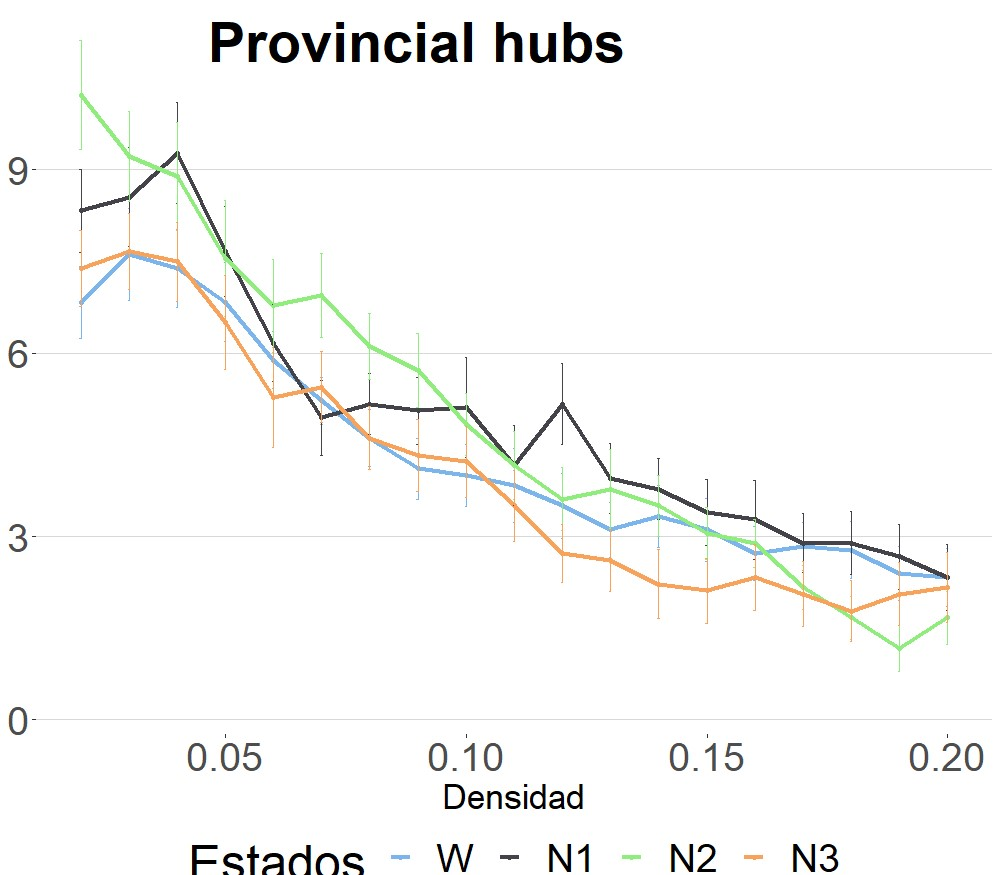
\includegraphics[width = 5in]{img/5_provincialhubs.jpg}
    \caption{Provincial Hubs}
    \label{fig:5_provincialhubs}
\end{figure}


\subsubsection{Provincial Nodes}
La cantidad de Provincial Nodes decrece con el incremento de la densidad para todos los estadíos del sueño y para el estado despierto. Se hallaron diferencias significativas para dos valores de baja densidad del comparativo de W con N1
y en un caso de baja densidad del comparativo de W con N2. En los dos puntos significativos el estadío de sueño presentó un número mayor de PN para ese valor de densidad. En los tres comparativos se observó el mismo comportamiento: el estadío del sueño comienza tomando valores superiores a W para bajas densidades y, a medida que se incrementa la densidad, a partir de 0.08 aproximadamente se invierte el orden y W toma valores más elevados que los estadíos del sueño.


\begin{figure}[H]
    \centering
    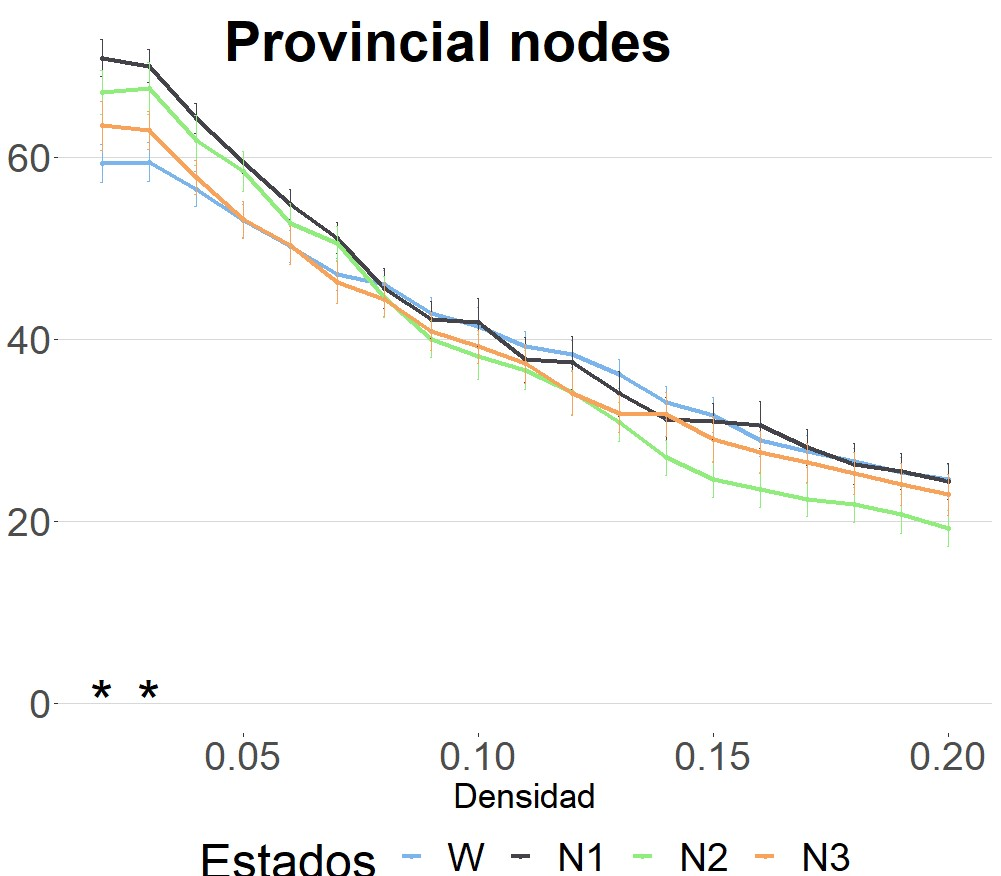
\includegraphics[width = 5in]{img/5_provincialnodes.jpg}
    \caption{Provincial Nodes}
    \label{fig:5_provincialnodes}
\end{figure}


\subsubsection{Visualizar para densidad 0.08}
A continuación fijando una densidad de 0.08, se hace una visualización de la red promedio binaria para cada estadío, discriminando los nodos según su rol. Se definió este nivel de densidad, ya que se probaron con varios, pero  para obtener una lectura más clara de las conexiones $0.08$ fue el que mejor resultado nos dio ya que a medida que se aumentaba la densidad las conexiones se hacían más complejas de describir, algo que notamos fue mayor cambio a central nodes en la región parietal.

\begin{figure}[H]
    \centering
    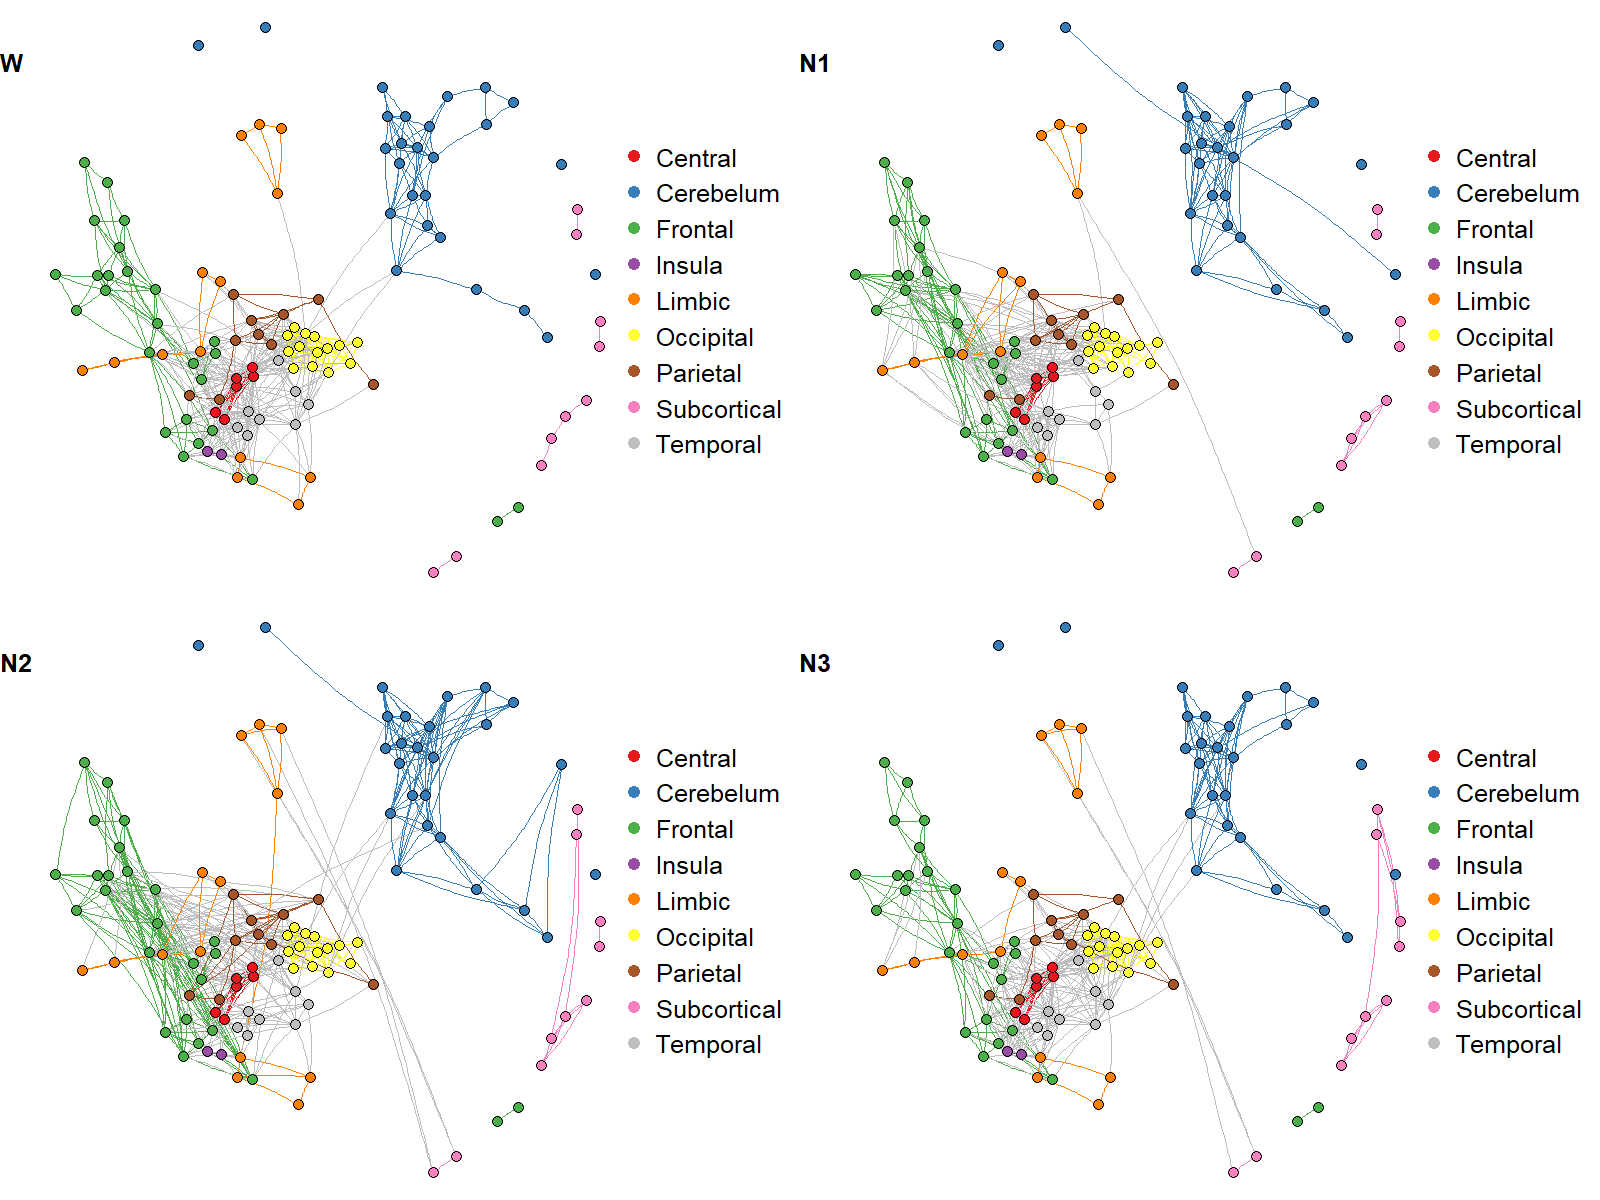
\includegraphics[width=\textwidth]{img/5_redescerebro_008.png}
    \caption{Zonas del Cerebro}
    \label{fig:Ejer5_redescerebro_008}
\end{figure}

\begin{figure}[H]
    \centering
    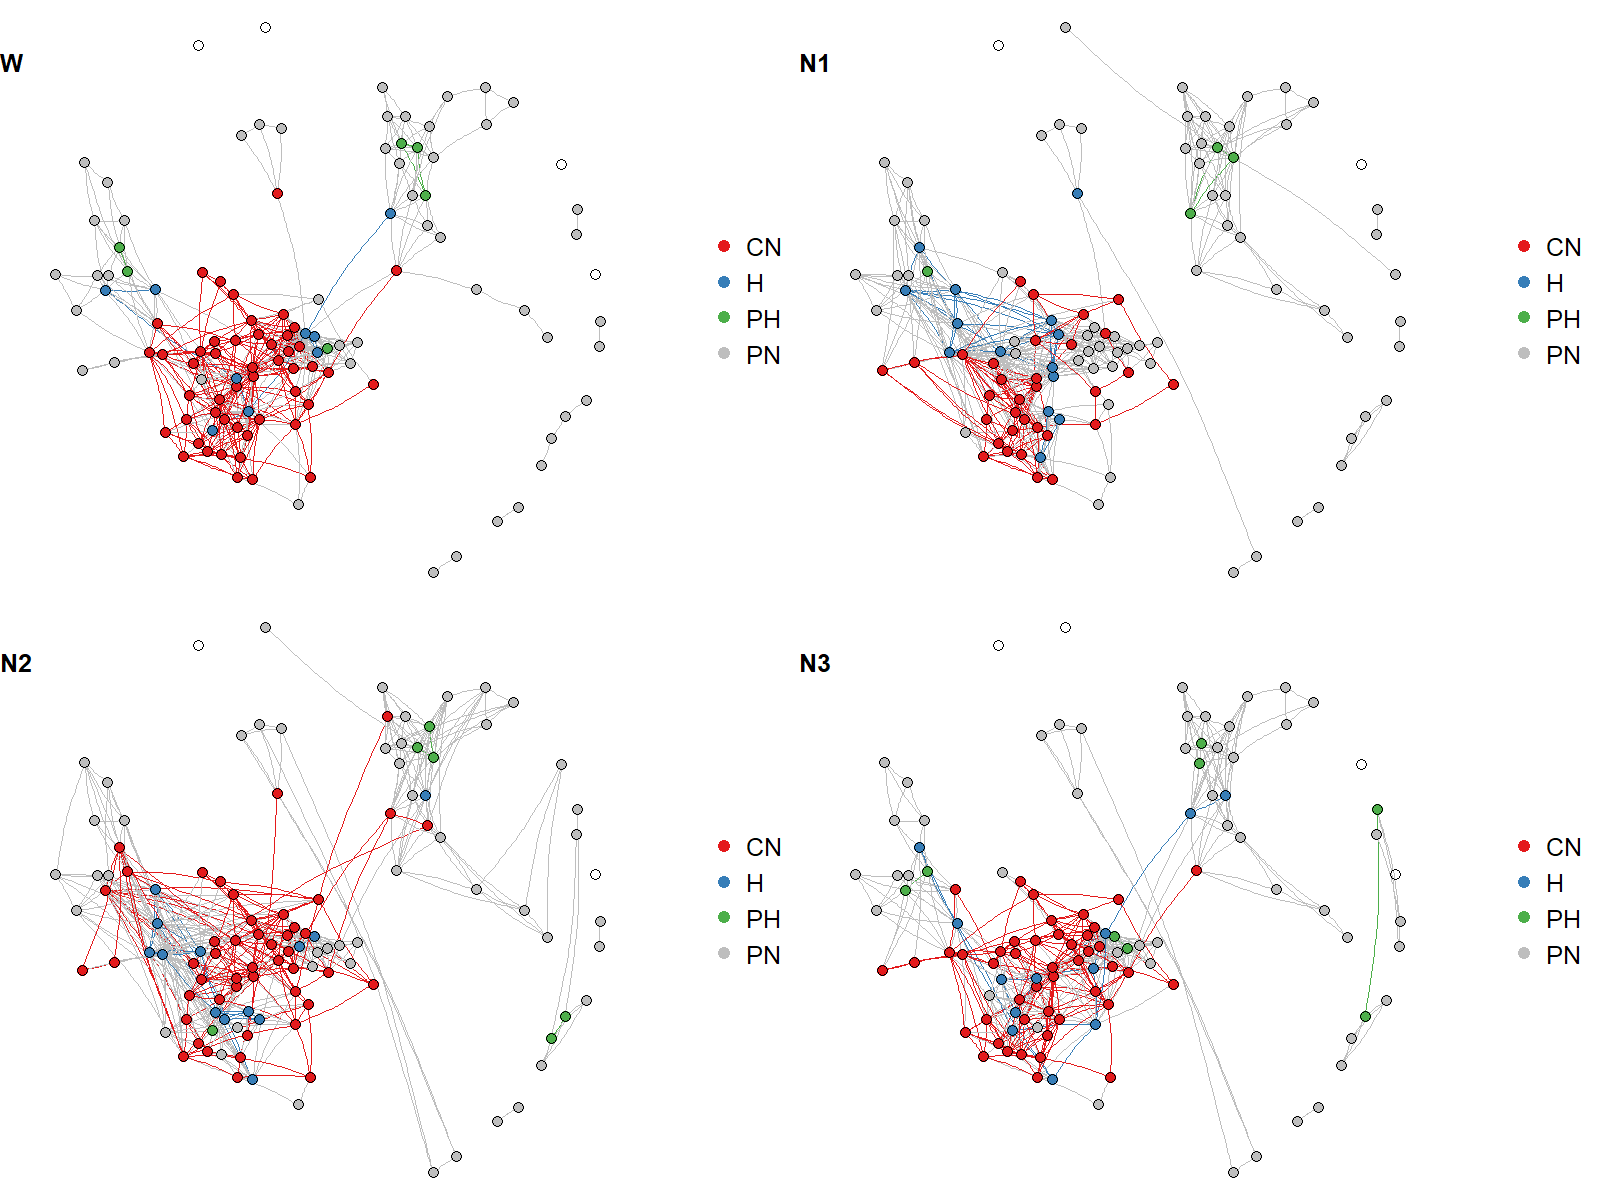
\includegraphics[width=\textwidth]{img/5_redes_roles008.png}
    \caption{Roles con Densidad 0.08}
    \label{fig:Ejer5_redes_roles008}
\end{figure}

No observamos claramente la relación entre agrupamientos funcionales y anatómicos sin embargo podemos concluir lo siguiente:

\begin{itemize} 
\item Para todos los estadíos del sueño la región (anatómica) Subcortical corresponde con Provincial Nodes (PN).
\item Para todos los estadíos del sueño casi toda la región (anatómica) Cerebelum corresponde con PN, aunque presenta algunos Hubs (H) y Provincial Hubs (PH)
\item La región anatómica Insula varía su comportamiento en cada estadío del sueño. Para los estados N1 y N2 se compone únicamente de Central Nodes (CN), en el estadío N3 de H y en el W de PN.
\item No observamos ningún patrón relevante para el resto de las regiones del cerebro debido a  que presentan varios tipos distintos de nodos en todos los estadíos y los mismos sufren modificaciones sin un patrón claro.
\end{itemize}

\printbibliography

\end{document}

